\section{Data Understanding}
\textbf{Acquisition protocol.} \fillme{Participants, anonymization, back-pocket placement, accelerometer/gravity/gyroscope configuration, number/duration/terrain of rides, and source organization.}

\textbf{Quality screening.} \fillme{Show measured sampling rates; document exclusion of participant \#03 (~62 Hz, Nyquist ~31 Hz, incompatible with 40--46 Hz features). Describe what this does to participant generalizability.}

\textbf{Available independent units.} \fillme{State both number of windows and independent original recording/session groups; identify how Raw031--Raw041 map to two parent sessions.}

\subsection{Empirical Measurements - Road Frequency versus Leg Movement Artifacts}
It was decided to conduct an experiment to evaluate whether there was a possible overlap with low frequency artifacts (such as leg movements) with the natural vibration caused by the gaps on the road.

Accordingly, an empirical experiment was carried out to empirically measure those frequencies.

\begin{figure}[htbp]
    \centering
    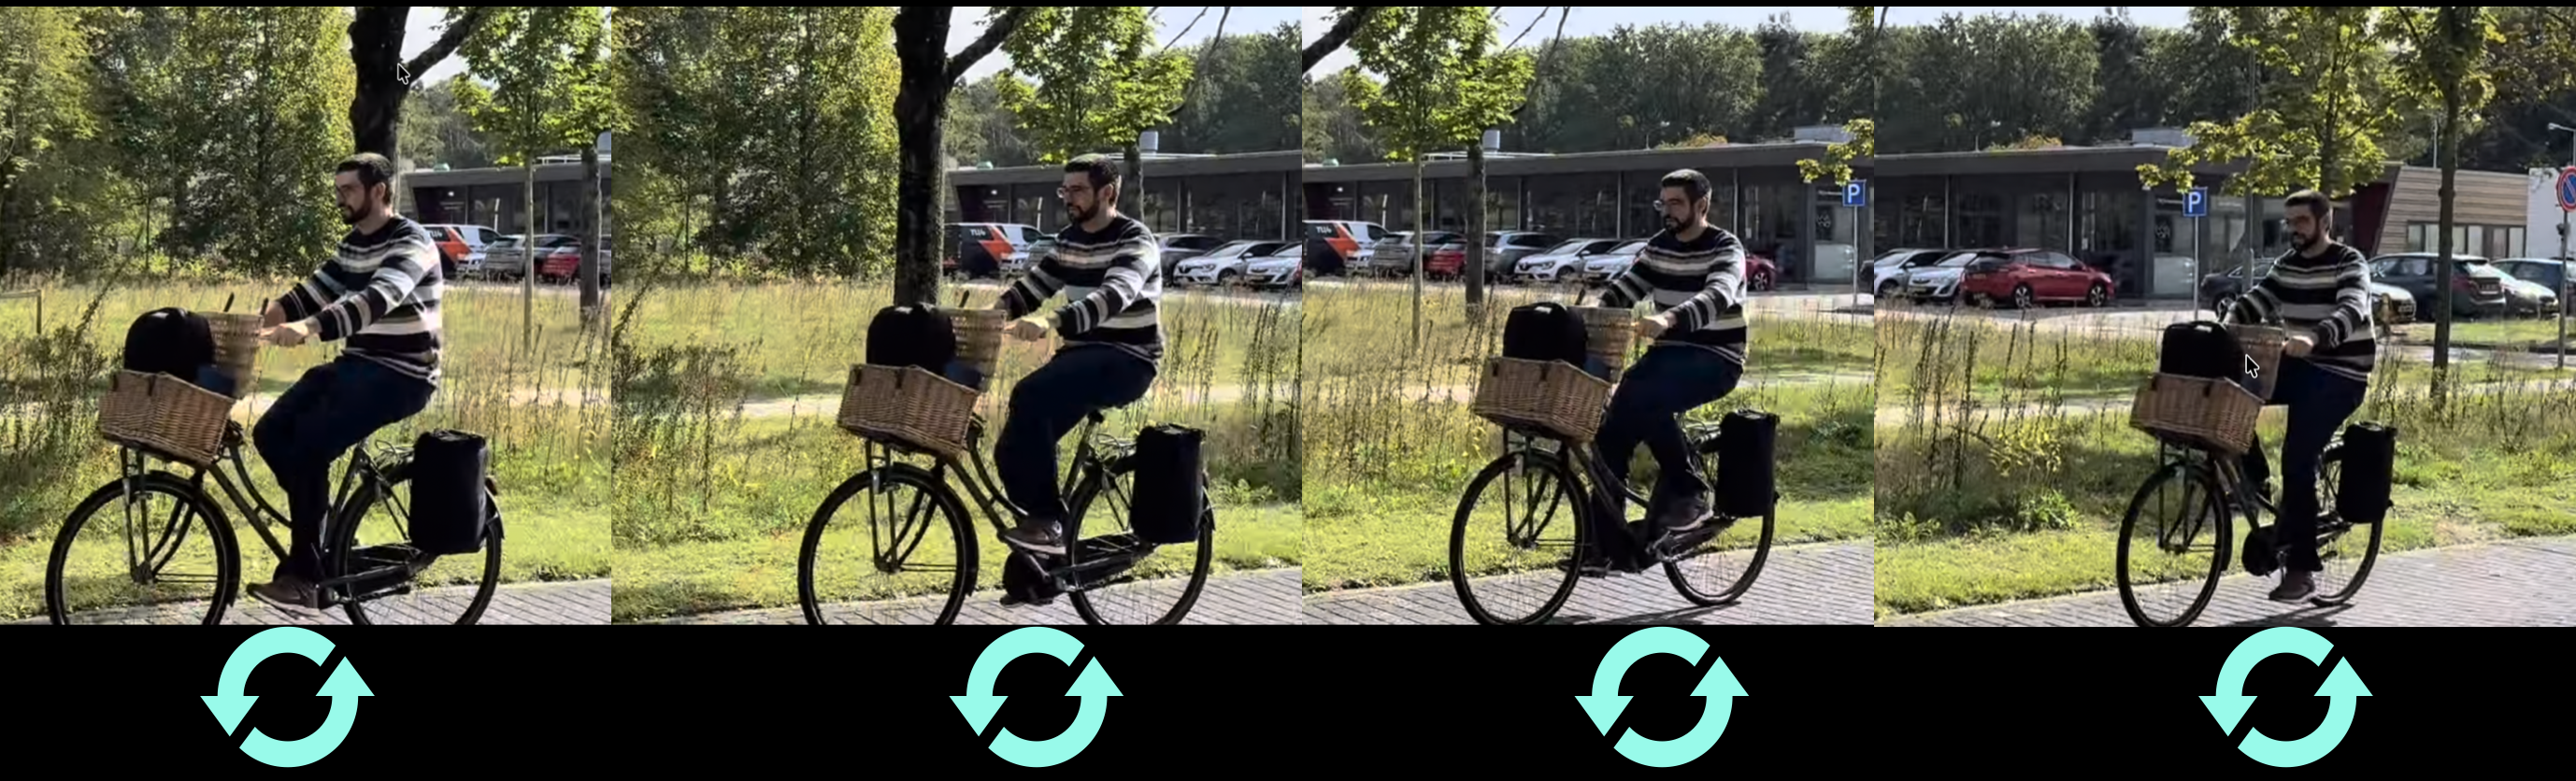
\includegraphics[width=0.8\linewidth]{figures/leg-movement}
    \caption{Example of manually counting the rotations per minute based on the video recording from one of the participants.}
    \label{fig:leg-mov}
\end{figure}

\begin{figure}[htbp]
    \centering
    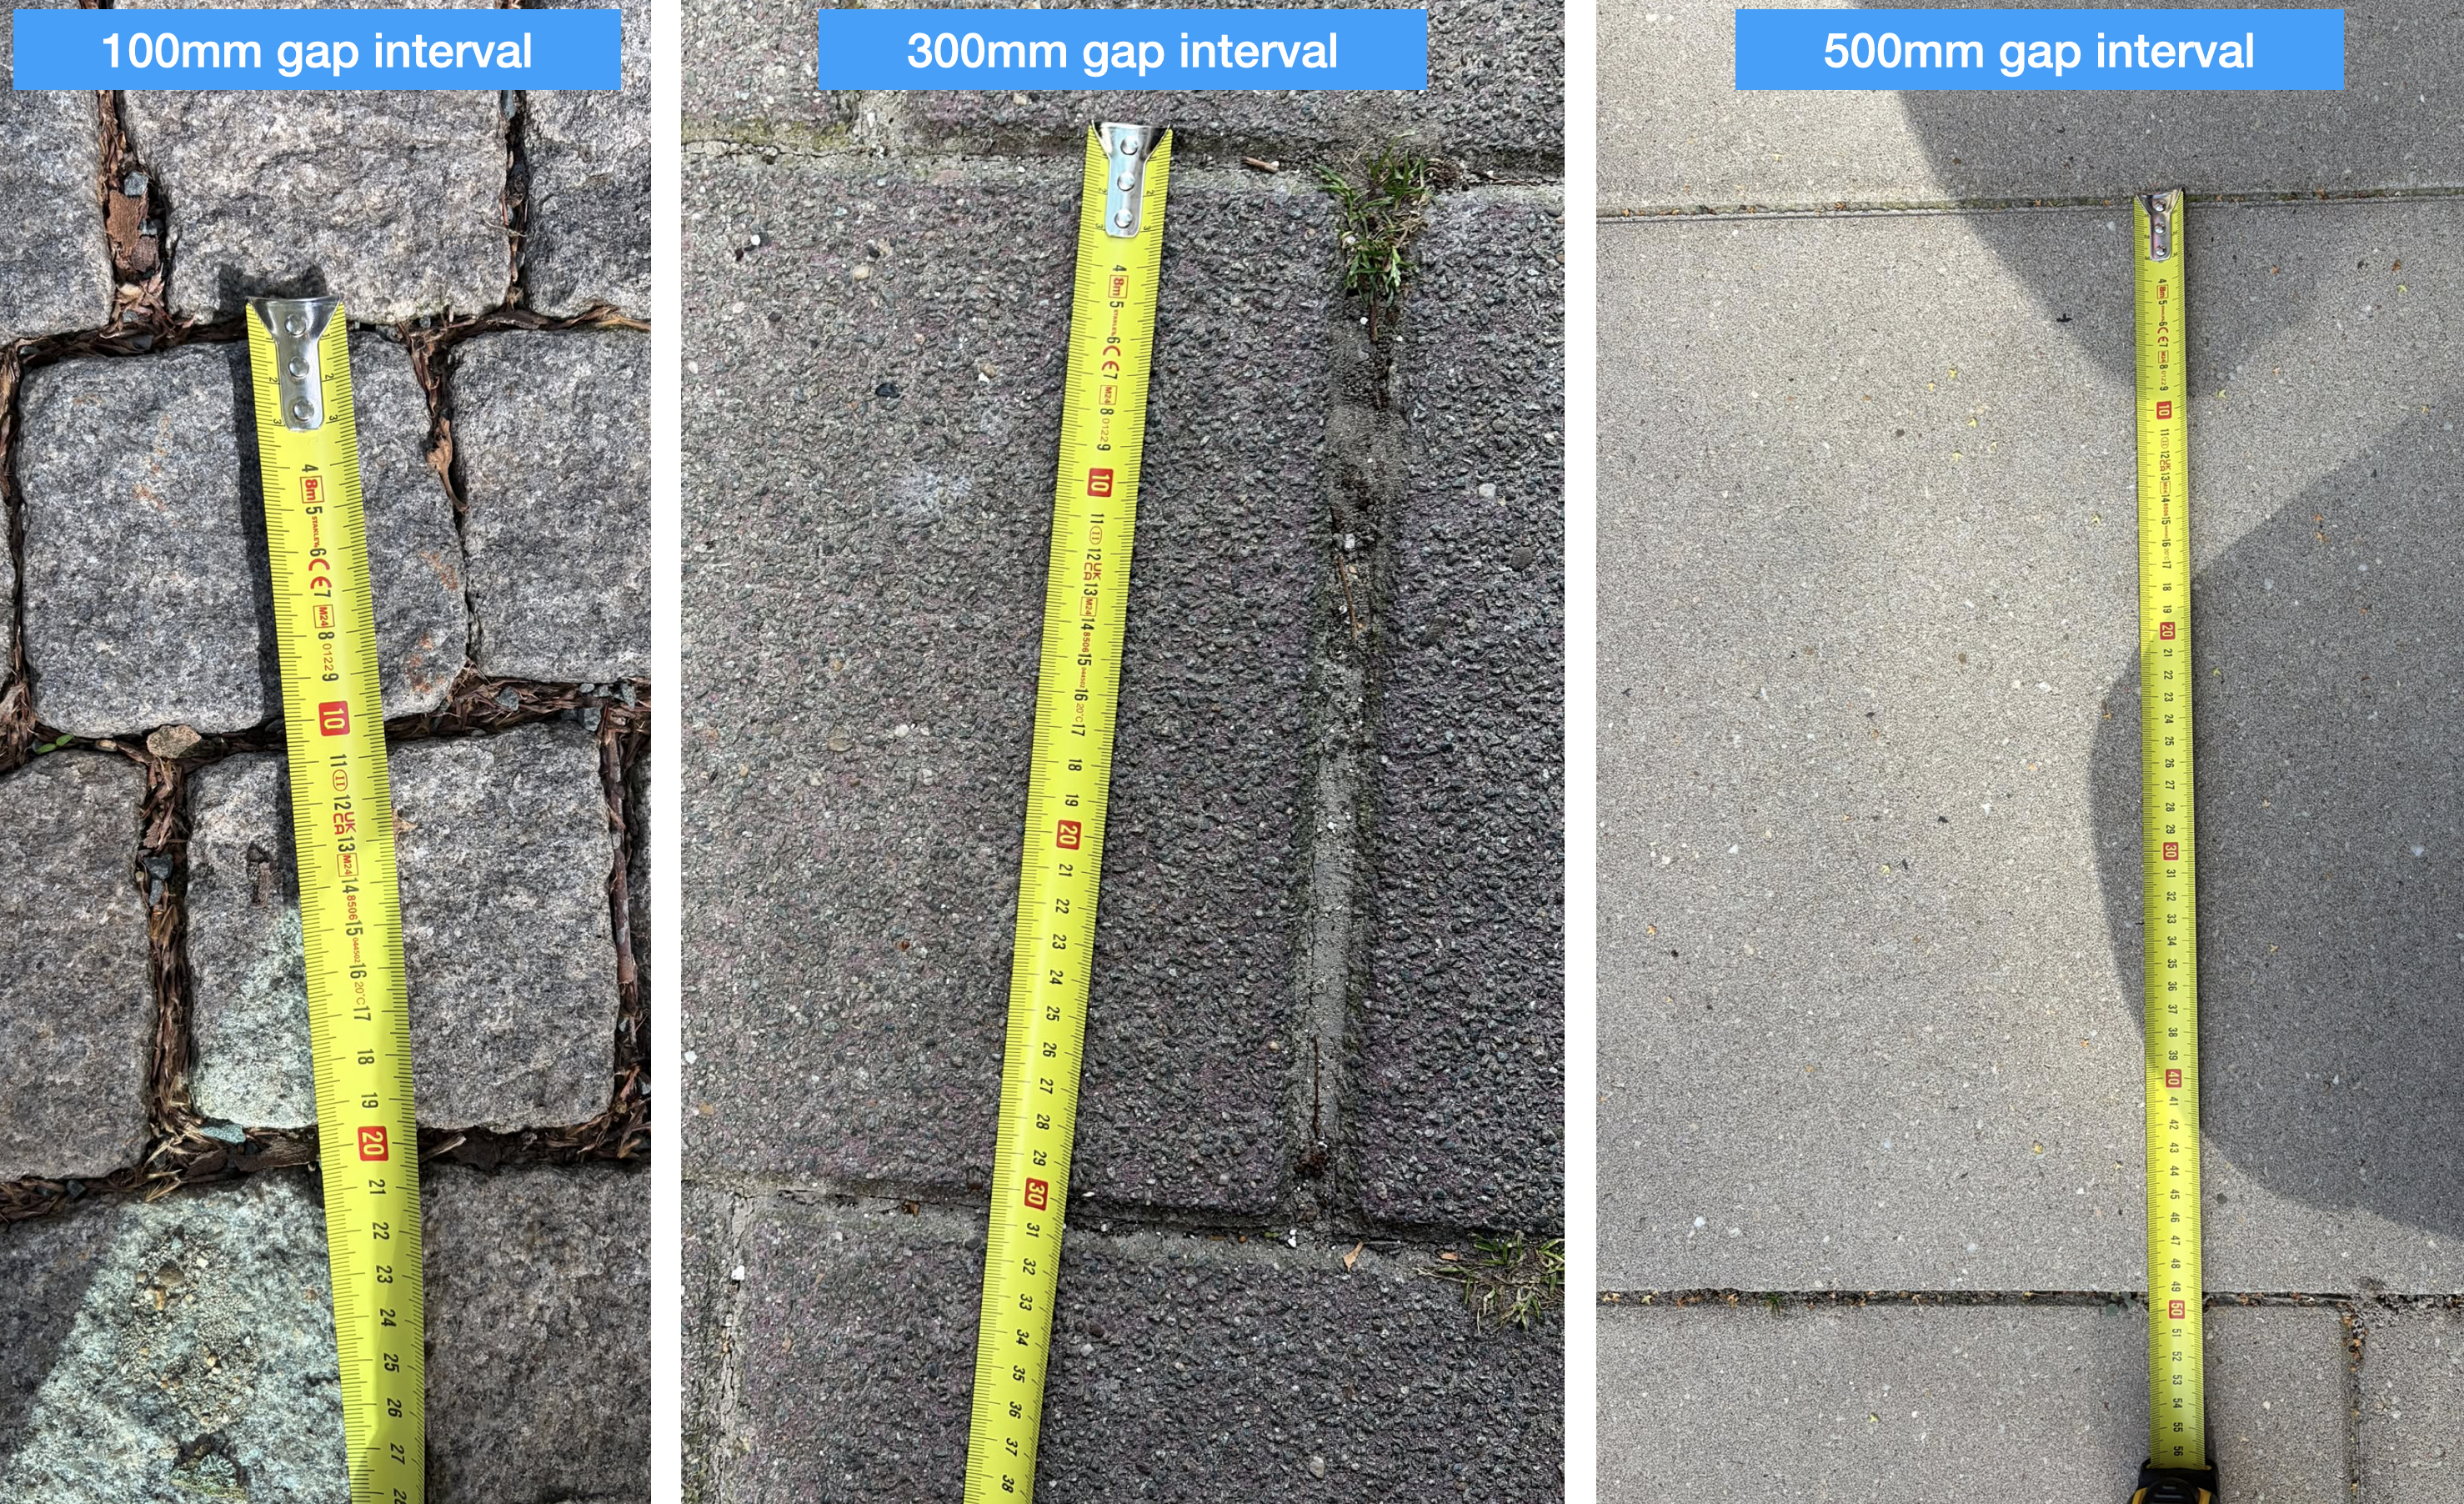
\includegraphics[width=0.8\linewidth]{figures/gap-bumpy-terrain}
    \caption{Different types of bumpy terrains were considered. The measured terrains ranged from $100 \sim 500mm$ gap interval.}
    \label{fig:road-gaps}
\end{figure}


The approximate road-excitation frequency was estimated from the measured
cycling velocity and the spatial spacing between terrain irregularities:

\begin{equation}
    f_{\text{road}} \approx \frac{v}{\lambda},
\end{equation}

where $v$ is the bicycle velocity and $\lambda$ is the spatial terrain
spacing. For the experiment, $\lambda = 100$ mm $= 0.1$ m. The bicycle
velocity was calculated from the travelled distance $d$ and the mean time
of the three repetitions:

\begin{equation}
    v = \frac{d}{\bar{t}}.
\end{equation}

Pedalling frequency was estimated by manually counting complete leg-motion
cycles over a measured video duration:

\begin{equation}
    f_{\text{pedal}} = \frac{N_{\text{cycles}}}{t},
\end{equation}

with cadence expressed in revolutions per minute as

\begin{equation}
    \mathrm{RPM} = 60 f_{\text{pedal}}.
\end{equation}

\begin{table}[htbp]
    \centering
    \caption{Measured cycling speed and estimated road-excitation frequency for a terrain spacing of $\lambda = 100$ mm.}
    \label{tab:road_frequency}
    \begin{tabular}{ccccccccc}
        \toprule
        $\lambda$ 
        & Distance
        & Intended
        & $t_1$
        & $t_2$
        & $t_3$
        & $\bar{t}$
        & Speed
        & $f_{\text{road}}$ \\
        (mm)
        & (m)
        & speed
        & (s)
        & (s)
        & (s)
        & (s)
        & (m/s)
        & (Hz) \\
        \midrule
        100 & 10 & Slow   & 3.63 & 4.06 & 4.03 & 3.91 & 2.56 & 25.60 \\
        100 & 10 & Medium & 2.50 & 2.45 & 2.60 & 2.52 & 3.97 & 39.74 \\
        100 & 10 & Fast   & 1.95 & 1.85 & 2.06 & 1.95 & 5.12 & 51.19 \\
        \bottomrule
    \end{tabular}
    \label{tab:road-freq}
\end{table}

As shown in table \ref{tab:road-freq}, the data was calculated for a gap interval $\lambda = 100mm$. As it can be seen in figure \ref{fig:road-gaps}, we can easily extrapolate those results with $\lambda=300mm$ and $\lambda=500mm$.

We already know the higher end of the spectrum, with $\lambda = 100mm$ at maximum speeds, which yields a road frequency of $\approx 51Hz$. To estimate to the best of our abilities the other side of the spectrum, we need to consider the maximum gap measured ($\lambda = 500mm$), associated with the slowest speed in table \ref{tab:road-freq} ($\approx 2.5 m/s$) which will, in turn, result in a minimum road frequency of $\approx 5Hz$.


\begin{table}[htbp]
    \centering
    \caption{Estimated pedalling cadence from manually counted leg-motion cycles.}
    \label{tab:pedalling_frequency}
    \begin{tabular}{lcccc}
        \toprule
        Video
        & Duration
        & Cycles counted
        & $f_{\text{pedal}}$
        & Cadence \\
        & (s)
        &
        & (Hz)
        & (RPM) \\
        \midrule
        rpm-video-1.mp4 & 17 & 26 & 1.53 & 91.76 \\
        rpm-video-2.mp4 & 21 & 30 & 1.43 & 85.71 \\
        rpm-video-3.mp4 & 25 & 30 & 1.20 & 72.00 \\
        \bottomrule
    \end{tabular}
    \label{tab:leg-rpm}
\end{table}

Based on the results computed in table \ref{tab:leg-rpm}, it is clear important to observe that we're only interested in the highest possible speed, and that is why the group participant was request to cycle as fast as possible. Since a single gear bicycle was used in the experiment, one could claim that the number of leg revolutions would be as high as possible and still, the maximum frequency observed was still under $2 Hz$.

The combined results of both experiments offer a solid base for the intuition that there seems to be, indeed, a gap in the frequency spectrum of the leg movements and the road vibration frequency. 



\figorplaceholder{figures/sampling_rates.pdf}{0.76}{Measured sampling-rate checks across the acquired recordings.}{fig:sampling}
